\documentclass[12pt]{article}
\usepackage{graphicx}
\usepackage{geometry}
\usepackage{fancyhdr}
\usepackage{titletoc}
\usepackage{titlesec}
\usepackage{listings}

% Page setup
\geometry{
    top=1in,
    bottom=1in,
    left=1in, % Adjust the left margin
    right=1in, % Adjust the right margin
}

% breaklines=true,

\pagestyle{fancy}
\fancyhf{} % Clear all header and footer fields
\fancyhead[R]{Evolutionary Algorithms} % Add this line to set the header on the right side
\renewcommand{\headrulewidth}{0pt} % Remove the horizontal line in the header

% Define section numbering format
\titleformat{\section}{\normalfont\large\bfseries}{\thesection}{1em}{}
\titleformat{\subsection}{\normalfont\normalsize\bfseries}{\thesubsection}{1em}{}

% Title Page
\begin{document}
\begin{titlepage}
    \centering
    {\LARGE\textbf{CS 451 : Computational Intelligence}\par}
    \vspace{0.5cm}
    {\Large Assignment 1\par}
    \vspace{0.2cm}
    {\Large Evolutionary Algorithms\par}
    \vspace*{\fill} % Vertically center the logo and text
    {\large Mustafa Sohail $\mid$ ms06860@st.habib.edu.pk\par}
    {\large Muhammad Azeem Haider $\mid$ mh06858@st.habib.edu.pk\par}
    \vspace{2cm}
    
\includegraphics[height=7cm]{images/HU_logo}\\\bigskip
    {\large \today}\\\bigskip\bigskip
    \vspace{1cm}
    \vspace{2cm}
    {\large Dhanani School of Science and Engineering\par}
    {\large Habib University\par}
    {\large Fall 2023\par}
    \vspace*{\fill} % Vertically center the copyright text
    {\large Copyright @ 2023 Habib University\par}
\end{titlepage}

% Index page
\thispagestyle{empty} % No page number on index page
\tableofcontents
\clearpage

\section{Introduction}
The first assignment of the course Computational Intelligence (CS-451) required us to implement evolutionary algorithms for three problems which are as followed:

\begin{enumerate}
    \item \textbf{Travelling Salesman Problem:} The Travelling Salesman Problem (TSP) is a classic problem in combinatorial optimization. It is the problem of finding a tour of a set of n cities that is of minimum cost. A tour is a permutation of the cities, and the cost of a tour is the sum of the distances between adjacent cities in the tour.
    \item \textbf{Job-Shop Scheduling Problem:} The job-shop scheduling problem is a classic problem in combinatorial optimization. It is the problem of scheduling a set of n jobs on a set of m machines. Each job consists of a sequence of operations, each of which must be processed on a specific machine for a specific amount of time.
    \item \textbf{Evolutionary Art (Mona Lisa):} The evolutionary art problem is a classic problem in evolutionary computation. It is the problem of evolving a population of images to match a target image. Each image in the population is represented as a string of genes, and the fitness of an image is the similarity between the image and the target image.
\end{enumerate}

\section{Travelling Salesman Problem}

\subsection{Problem Formulation}

The travelling salesman problem requires finding of the minimum cost (distance) to cover all the cities. The \textbf{chromosome generation} is being carried out by randomly shuffling the cities of the Qatar dataset. 
\newline \\
Furthermore, the \textbf{mutate function} assigns each chromosome a random number from 0 to 1, and if the number is less than the mutation rate, mutation occurs. 
\newline \\
Finally, the \textbf{crossover function} once again, carries out crossover between two parents by assigning the crossover point, and all the repeated cities from the second parent, that are already added in the first part, are added linearly in the end. 

\subsection{Analysis}

While carrying out initial combination for selection schemes for parent selection and survival selection, it was clear that a combination of an explorative scheme as a parent selection and an exploitative scheme as a survival selection would be the best. As a result, two main combinations that were tested were the following:

    \begin{enumerate}
        \item \textbf{Parent Selection:} Random \textbf{Survival Selection:} truncation
        \item \textbf{Parent Selection:} tournament selection \textbf{Survival Selection:} truncation
    \end{enumerate}

% We yeilded the following result for the first combination, where we had two extremes as the parent selection and survival selection schemes:

% \begin{center}
\begin{figure}[h]
    \centering
    \includegraphics[width=0.65\textwidth]{images/figure_1.png}
    \caption{Travelling Salesman Problem: Combination 1}
\end{figure}
% \end{center}

The result reported in \textit{Figure 1}, was obtained by the following parameters:

\begin{enumerate}
    \item \textbf{Population Size:} 1000
    \item \textbf{Offspring Size:} 200
    \item \textbf{Number of Generations:} 5000
    \item \textbf{Mutation Rate:} 0.45
    \item \textbf{Iterations:} 10
\end{enumerate}


\section{Job-Shop Scheduling Problem}

\subsection{Problem Formulation}

The job-shop scheduling problem requires finding the minimum time to complete all the jobs on all the machines.
\\ \newline
The chromosome is generated by providing each job with an index, and repeating that number of index for the number of operations on that job. For example for abz5, if there are 10 jobs with 10 operations each, each job will be given an index from 0-9 and each number from 0-9 will repeat exactly 10 times. In this manner, we have flattened our chromosome. 
\\ \newline
The mutate and crossover function work in similar fashion to the travelling salesman problem. The mutate function checks probability assigned and if it is less than mutation rate, mutation occurs, and crossover occurs between two parents, and repeated jobs from parent two are added in the end of the new offsprings. 

\subsection{Analysis}

Unlike, the travelling salesman problem, the job-shop scheduling problem had three input files which were abz(5-7). The analysis for each file will be divided into subsections.

\subsubsection{First input file ``abz5''}

The strategy to solve the job-shop scheduling problem was to use the same combination of parent selection and survival selection as the travelling salesman problem. Since keeping the parent selection scheme entirely explorative through \textit{random} function or on the higher exploration through rank-based selection or tournament selection. The survival selection was to be kept entirely exploitative through truncation or on the higher exploitation through fitness proportional selection. The best score achieved \textbf{1242} was through \textbf{random} and \textbf{truncation}, with the following parameters. 

\begin{enumerate}
    \item \textbf{Population Size:} 200
    \item \textbf{Offspring Size:} 60
    \item \textbf{Number of Generations:} 2000
    \item \textbf{Mutation Rate:} 0.5
    \item \textbf{Iterations:} 10
\end{enumerate}

\begin{figure}[h]
    \centering
    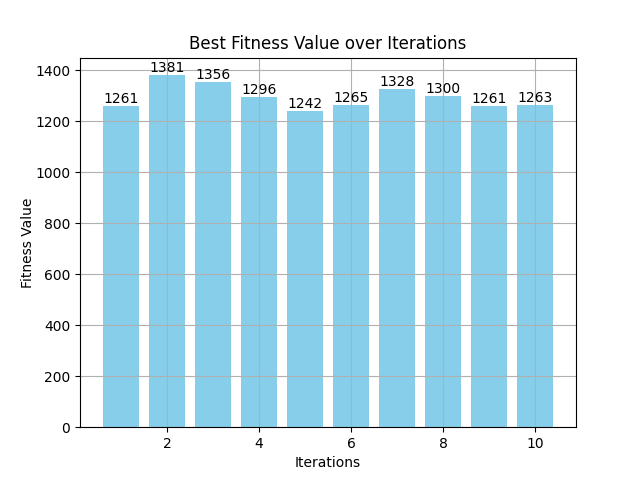
\includegraphics[width=0.65\textwidth]{images/Figure_2.png}
    \caption{Job-shop Scheduling Problem: Combination 1}
\end{figure}

The ratio between population size and offsprings was tinkered with as well as the value of mutation rate. 
Other combinations of schemes such as rank-based selection as parent selection and truncation as survival selection yielded the following result, \textbf{1253} which came very close to our best score. 

\begin{figure}[h]
    \centering
    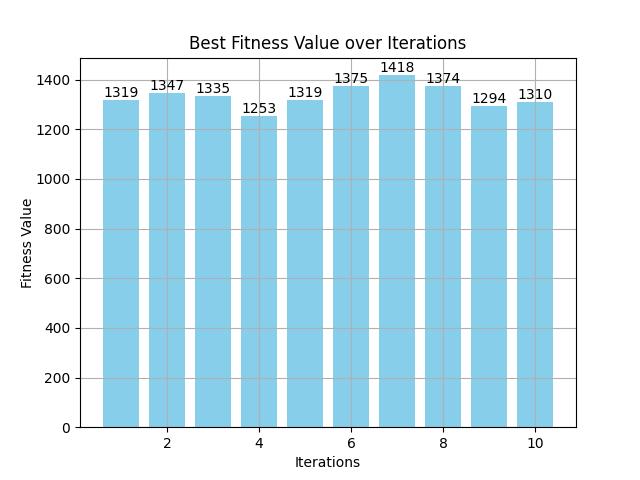
\includegraphics[width=0.65\textwidth]{images/JSSP_rbstr150-40-2000-0.5-10.png}
    \caption{Job-shop Scheduling Problem: Combination 2}
\end{figure}

The following parameters were used to achieve the result in \textit{Figure 3}:

\begin{enumerate}
    \item \textbf{Population Size:} 150
    \item \textbf{Offspring Size:} 40
    \item \textbf{Number of Generations:} 2000
    \item \textbf{Mutation Rate:} 0.5
    \item \textbf{Iterations:} 10
\end{enumerate}

\subsubsection{Input files ``abz6'' and ``abz7''}

The combination of schemes for both the input files are random and truncation with the following parameters:

\begin{enumerate}
    \item \textbf{Population Size:} 1000
    \item \textbf{Offspring Size:} 200
    \item \textbf{Number of Generations:} 500
    \item \textbf{Mutation Rate:} 0.45
    \item \textbf{Iterations:} 10
\end{enumerate}

The best score for the input file ``abz6'' was \textbf{972}. Whereas, the best score for the input file ``abz7'' was \textbf{776}. The reason for the scores of input file ``abz6'' and ``abd7'' being lower than the input ``abz5'' is due to the fact that the time needed by each process on each machine is significantly low. 

\begin{figure}[h]
    \centering
    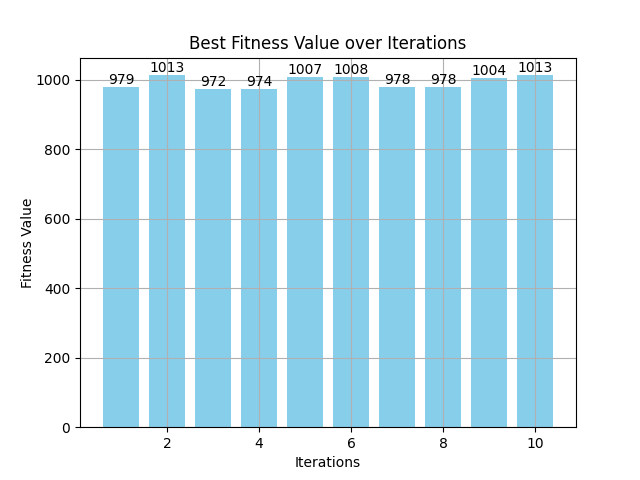
\includegraphics[width=0.6\textwidth]{images/abz6_rntr1000-200-500-0.45-10.png}
    \caption{Job-shop Scheduling Problem: Input file abz6}
\end{figure}

\begin{figure}[h]
    \centering
    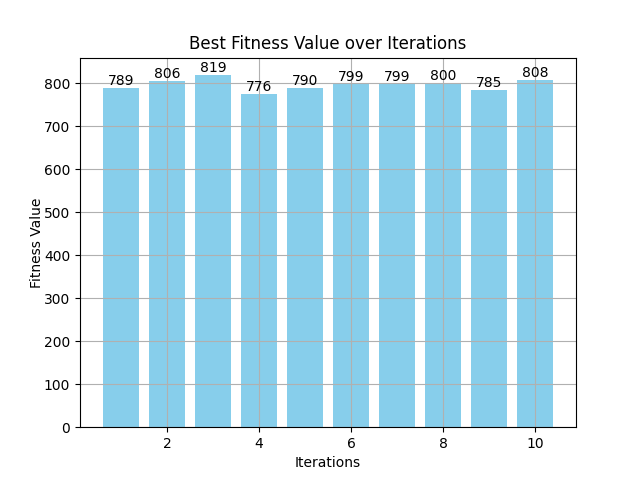
\includegraphics[width=0.6\textwidth]{images/abz7_rntr1000-200-500-0.45-10.png}
    \caption{Job-shop Scheduling Problem: Input file abz7}
\end{figure}

\section{Evolutionary Art: Mona Lisa}

\end{document}